\def\year{2020}\relax
%File: formatting-instruction.tex
\documentclass[letterpaper]{article} % DO NOT CHANGE THIS
\usepackage{aaai20}  % DO NOT CHANGE THIS
\usepackage{times}  % DO NOT CHANGE THIS
\usepackage{helvet} % DO NOT CHANGE THIS
\usepackage{courier}  % DO NOT CHANGE THIS
\usepackage[hyphens]{url}  % DO NOT CHANGE THIS
\usepackage{graphicx} % DO NOT CHANGE THIS
\input{idp-latex/idp-latex}
\setboolean{commentmargin}{false}
\newcommand{\tias}[1]{\namedcomment{#1}{tg}{purple}}
\newcommand{\jens}[1]{\namedcomment{#1}{jc}{brown}}
\newcommand{\rocs}[1]{\namedcomment{#1}{rc}{Sepia}}
\usepackage{paralist}


\usepackage{tikz}
\usepackage{textcomp}
\usetikzlibrary{shapes,arrows}

\urlstyle{rm} % DO NOT CHANGE THIS
\def\UrlFont{\rm}  % DO NOT CHANGE THIS
\usepackage{graphicx}  % DO NOT CHANGE THIS
\frenchspacing  % DO NOT CHANGE THIS
\setlength{\pdfpagewidth}{8.5in}  % DO NOT CHANGE THIS
\setlength{\pdfpageheight}{11in}  % DO NOT CHANGE THIS
\nocopyright %TODO REMOVE IF THIS EVER GOES TO AAAI OR SOMETHING OF THE KIND USING AAAI STYLE
% \usepackage{tikz} 
\newcommand{\citet}[1]{\citeauthor{#1}~(\citeyear{#1})}
%PDF Info Is REQUIRED.
% For /Author, add all authors within the parentheses, separated by commas. No accents or commands.
% For /Title, add Title in Mixed Case. No accents or commands. Retain the parentheses.
 \pdfinfo{
/Title (TODO TITLE) % TODO
/Author (TODO AUTHORS) % TODO
} %Leave this	
% /Title ()
% Put your actual complete title (no codes, scripts, shortcuts, or LaTeX commands) within the parentheses in mixed case
% Leave the space between \Title and the beginning parenthesis alone
% /Author ()
% Put your actual complete list of authors (no codes, scripts, shortcuts, or LaTeX commands) within the parentheses in mixed case. 
% Each author should be only by a comma. If the name contains accents, remove them. If there are any LaTeX commands, 
% remove them. 

% DISALLOWED PACKAGES
% \usepackage{authblk} -- This package is specifically forbidden
% \usepackage{balance} -- This package is specifically forbidden
% \usepackage{caption} -- This package is specifically forbidden
% \usepackage{color (if used in text)
% \usepackage{CJK} -- This package is specifically forbidden
% \usepackage{float} -- This package is specifically forbidden
% \usepackage{flushend} -- This package is specifically forbidden
% \usepackage{fontenc} -- This package is specifically forbidden
% \usepackage{fullpage} -- This package is specifically forbidden
% \usepackage{geometry} -- This package is specifically forbidden
% \usepackage{grffile} -- This package is specifically forbidden
% \usepackage{hyperref} -- This package is specifically forbidden
% \usepackage{navigator} -- This package is specifically forbidden
% (or any other package that embeds links such as navigator or hyperref)
% \indentfirst} -- This package is specifically forbidden
% \layout} -- This package is specifically forbidden
% \multicol} -- This package is specifically forbidden
% \nameref} -- This package is specifically forbidden
% \natbib} -- This package is specifically forbidden -- use the following workaround:
% \usepackage{savetrees} -- This package is specifically forbidden
% \usepackage{setspace} -- This package is specifically forbidden
% \usepackage{stfloats} -- This package is specifically forbidden
% \usepackage{tabu} -- This package is specifically forbidden
% \usepackage{titlesec} -- This package is specifically forbidden
% \usepackage{tocbibind} -- This package is specifically forbidden
% \usepackage{ulem} -- This package is specifically forbidden
% \usepackage{wrapfig} -- This package is specifically forbidden
% DISALLOWED COMMANDS
% \nocopyright -- Your paper will not be published if you use this command
% \addtolength -- This command may not be used
% \balance -- This command may not be used
% \baselinestretch -- Your paper will not be published if you use this command
% \clearpage -- No page breaks of any kind may be used for the final version of your paper
% \columnsep -- This command may not be used
% \newpage -- No page breaks of any kind may be used for the final version of your paper
% \pagebreak -- No page breaks of any kind may be used for the final version of your paperr
% \pagestyle -- This command may not be used
% \tiny -- This is not an acceptable font size.
% \vspace{- -- No negative value may be used in proximity of a caption, figure, table, section, subsection, subsubsection, or reference
% \vskip{- -- No negative value may be used to alter spacing above or below a caption, figure, table, section, subsection, subsubsection, or reference

\setcounter{secnumdepth}{1} %May be changed to 1 or 2 if section numbers are desired.

% The file aaai20.sty is the style file for AAAI Press 
% proceedings, working notes, and technical reports.
%
\setlength\titlebox{2.5in} % If your paper contains an overfull \vbox too high warning at the beginning of the document, use this
% command to correct it. You may not alter the value below 2.5 in
%\title{Towards End-To-End Solving and Explaining of Logic Grid Puzzles}
\title{User-oriented Solving and Explaining \\of Natural Language Logic Grid Puzzles}
%Your title must be in mixed case, not sentence case. 
% That means all verbs (including short verbs like be, is, using,and go), 
% nouns, adverbs, adjectives should be capitalized, including both words in hyphenated terms, while
% articles, conjunctions, and prepositions are lower case unless they
% directly follow a colon or long dash
% \author{Written by AAAI Press Staff\textsuperscript{\rm 1}\thanks{Primarily Mike Hamilton of the Live Oak Press, LLC, with help from the AAAI Publications Committee}\\ \Large \textbf{AAAI Style Contributions by
% Pater Patel Schneider,} \\ \Large \textbf{Sunil Issar, J. Scott Penberthy, George Ferguson, Hans Guesgen}\\ % All authors must be in the same font size and format. Use \Large and \textbf to achieve this result when breaking a line
% \textsuperscript{\rm 1}Association for the Advancement of Artificial Intelligence\\ %If you have multiple authors and multiple affiliations
% % use superscripts in text and roman font to identify them. For example, Sunil Issar,\textsuperscript{\rm 2} J. Scott Penberthy\textsuperscript{\rm 3} George Ferguson,\textsuperscript{\rm 4} Hans Guesgen\textsuperscript{\rm 5}. Note that the comma should be placed BEFORE the superscript for optimum readability
% 2275 East Bayshore Road, Suite 160\\
% Palo Alto, California 94303\\
% publications20@aaai.org % email address must be in roman text type, not monospace or sans serif
% % }
\author{Jens Claes\textsuperscript{\rm 1}, Bart Bogaerts\textsuperscript{\rm 2}, Rocsildes Canoy\textsuperscript{\rm 2}, Tias Guns\textsuperscript{\rm 2} \\
\textsuperscript{\rm 1} jensclaes33@gmail.com\\
\textsuperscript{\rm 2} Vrije Universiteit Brussel, firstname.lastname@vub.be %If you have multiple authors and multiple affiliations
}
 \begin{document}
 
 \newcommand\ourtool{\logicname{HolyZebra}}

\maketitle

\begin{abstract}
Inspired by the 2019 Holy Grail Challenge, we present \ourtool, a mostly automated tool that reads the natural language clues and a list of the entities of a logic grid puzzle (also known as Zebra puzzle). The challenge is to both handle the natural language input, and to produce a human-understandable explanation of how the solution is obtained.
We achieve this by translating the natural language clues into logic using a variation on the semantical framework of Blackburn and Bos. This logical representation is then used in a novel explanation-based reasoning procedure, on top of the \idp knowledge base system. The novelty is in the ordering based on mental effort required, which is related to the number of previously derived facts needed to derive new facts. The outcome is a stepwise visualisation of the clue(s) used and the resulting changes on the grid.
This can be used both to solve a puzzle, or as a step-wise `help' function for people stuck while solving a puzzle.

% \todo{choose name for system}

\end{abstract}

\section{Introduction}
Automated problem solving is central to the research field of Artificial Intelligence. A common assumption here is that the problem formulation is unambiguously specified as a problem specification (sometimes called \textit{model}) in a formal language. However, formulating such a specification is non-trivial, and for human beings it is much easier to specify problems in natural language.

Natural language processing (NLP) is studied as a proper subfield of AI~\cite{manning1999foundations}. Problem solving starting from natural language input has been studied for simple mathematical problems in the subfield of \textit{word problem solving} or natural language mathematical problems~\cite{Mukherjee2008}.

We here aim to study natural language combinatorial problems, both from human-produced input (e.g. natural language) and human-understandable output (in our case, visualisations), as per the Holy Grail 2019 challenge.\footnote{https://freuder.wordpress.com/pthg-19-the-third-workshop-on-progress-towards-the-holy-grail/} Generating human-understandable output to logic grid puzzles has initially been explored by \citet{sqalli1996inference}.

\paragraph{}
We present \ourtool,  an end-to-end solution for solving logic grid puzzles (also known as Zebra puzzles) and explaining in human-understandable terms how this solution can be obtained from the clues. 

\ourtool\footnote{\ourtool was originally developed in the context of a Master's thesis \cite{msc/Claes17}.} starts from a plain English language representation of the clues and a list of all the entities present in the puzzle. It then applies the standard NLP techniques to build a puzzle-specific \textit{lexicon}. This lexicon is fed into a type-aware variant of the semantical framework of Blackburn and Bos~(\citeyear{Blackburn2005,Blackburn2006}), which translates the clues into discourse representation theory \cite{DRT}. This logic is further transformed to a specification in the \idp language \mycite{idp}, an extension of first-order logic. 

It then uses this formal representation of the clues both to solve the puzzle and to explain the solution. 
There are many different ways in which such a system could explain itself. For instance, after finding a solution, it can explain \begin{inparaenum}\item \emph{why that is a solution} or \item \emph{why there are no other solutions}; additionally, it can explain \item \emph{how the system found this solution}, and \item \emph{how a human could find this solution}. \end{inparaenum}
 
Our system implements this last type of explanation. In contrast to how the system found the solution, it focuses on simplifying the explanation itself, rather than giving insights in the actual search algorithm used by \idp. As such, our explanations are not to be used for understanding the inner workings of the solver, but rather are to be used by people interested in solving logic puzzles.

In generating explanations and choosing the \textit{order} in which the reasoning steps are explained, we chose to order by an estimate of mental effort required to follow the reasoning step. Each reasoning step is visualised as the clue(s) involved and the resulting changes on the grid.

When solving such puzzels, it can either be used for explaining how to obtain an entire solution, or for providing help to users who are stuck during the solving process. Indeed, our explanation method will, given a partial solution, find the easiest next derivation to make. 

\todo{Perhaps too much of the system overview already in the intro...}\bart{Looks fine to me}




\section{System Overview}
\todo{Einstein puzzle as a running example? [T] if we call it holy zebra, makes sense to use Zebra as running example}



\ourtool takes as input a set of natural language sentences (from hereon referred to as ``clues'') and (optionally) domain information (names/values of the different entities in the problem domain).
In typical logic grid puzzles, this domain information is present in the grid. 
For some puzzles, domain information is not required; a prototypical example is Einstein's Zebra puzzle, which ends with the question ``who owns the zebra?'', while the puzzle can be solved without knowledge of the fact that there is a zebra in the first place. 
As we will detail below, for some puzzles, especially those with numeric values involved, this domain information is crucial to solving them. 

\ourtool then does this and this and that ... 

Figure \ref{fig:overview} contains an overview of the different components of the system.

\begin{figure*}
\centering
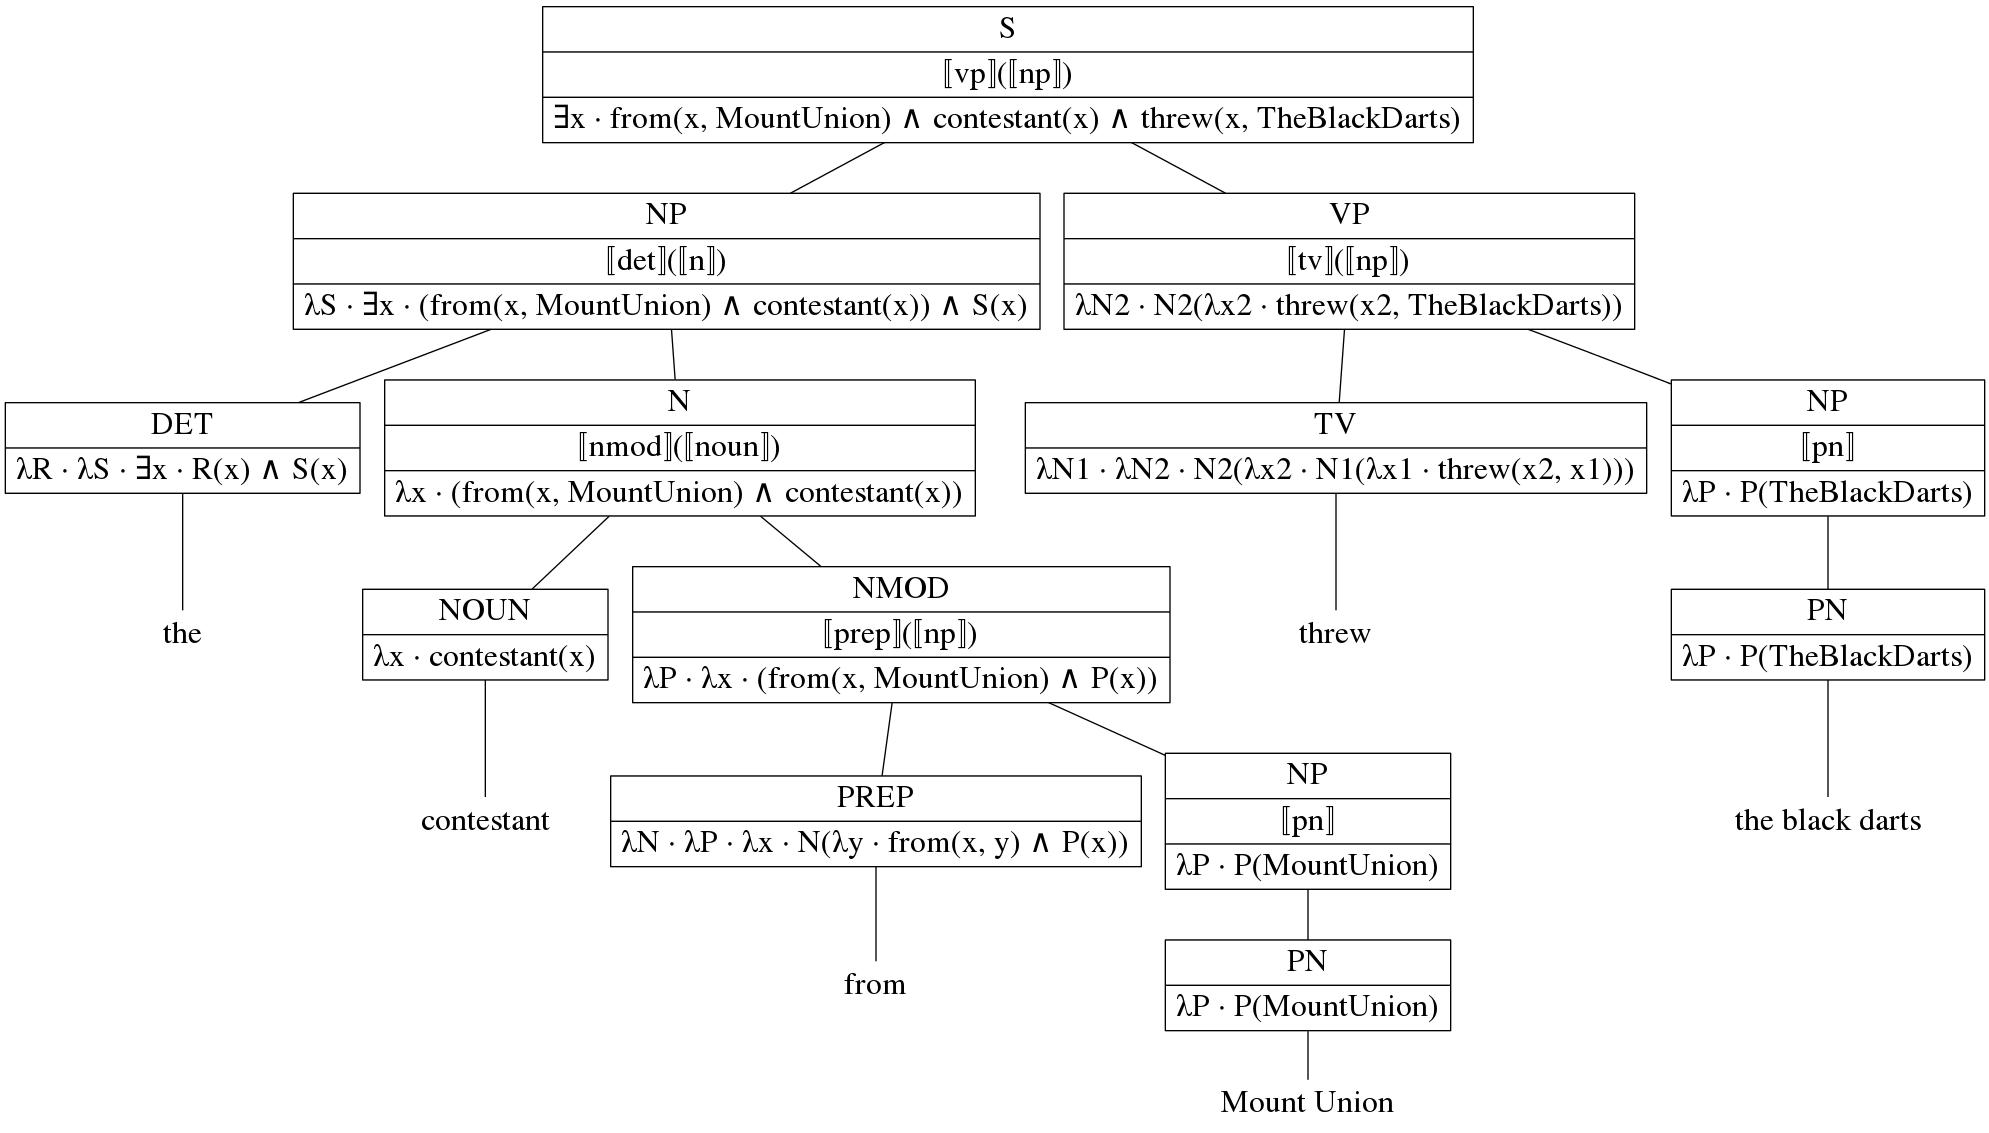
\includegraphics[width=\textwidth]{../../poster/graphviz/tree.jpg}
 Can someone replace this by a picture/schematic overview of the pipeline
 \caption{An overview of the pipeline of \ourtool.}
 \label{fig:overview}
\end{figure*}



\todo{
INCORPORTATE TEH FOLLOWING IN THE PAPER (Jens's description)}

\begin{verbatim}
0. Input
1. POS-tagger
2. POS-rewriter
3. Blackburn \& Bos
4. Transformer to IDP
5. IDP Lua Code
6. Glue code
7. Visualization
\end{verbatim}

\todo{
0. Input: take the input of the puzzle with the sentences and the different things splitted by type (e.g. \url{https://github.com/bartbog/holygrail/blob/master/data/a_bargain.json})

1. POS-tagger
Input: [0. Input]: the json (the clues)
Output: the POS-tags
This is a standard POS-tagger that will take the sentences from [0. Input] and will tag the different words with their Part of Speech tag

2. POS-rewriter
Input: [0. Input]: the json, [1. POS-tagger]: the POS-tags
Output: (A prolog fact with) the rewritten sentences and the problem-specific lexicon
Based on these POS-tags, the POS-rewriter will rewrite some sentences to better match the grammar used in [3. Blackburn \& Bos]. It will also derive the problem specific lexicon.

3. (Adapted) Blackburn \& Bos
Input: [2. POS-rewriter]: the prolog fact with the rewritten sentences and the problem-specific lexicon
Static input (same for all the problems): the grammar that was derived during my thesis, the semantincs of a word-type (e.g. a verb has meaning X), the semantics of a grammar rule (how to combine the meaning of the words in case those words appear as in the grammar rule). Some of these semantics were provided by Blackburn \& Bos, some were added because they were logic puzzle specific. 
E.g. a sentence of the form "Of X and Y, one A and the other B" is defined in \url{https://github.com/bartbog/holygrail/blob/master/bos/myGrammarSemantics.pl#L33} and \url{https://github.com/bartbog/holygrail/blob/master/bos/myGrammar.pl#L91-L100} and is logic puzzle specific
Output: 
 - The First Order Logic representation of all the sentences
 - (Because it's adapted to have types): The types of all the words in the sentences

Blackburn \& Bos is a general framework with 4 inputs: lexicon, grammar, semantics for the lexicon (per word SORT, not per word!), semantics for the grammar. It works by combining the semantics of the words in the way that the semantics of the grammar specifies. It uses Discourse Representation Theory (DRT) for this because this captures quantors way better + it would work across sentences (not used in logic puzzles but this could capture the "He" in "Bart went jogging. He is tired" as "Bart"). The framework also provides a way to translate the DRT to FOL.

Because I adapted the framework, we also get a type for every word. E.g. for "Bart works in Brussels", it knows the subject of "works in" needs to be of the same type as "Bart" and the object of the same type as "Brussels". 

4. Transformer to IDP:
Input: Ouputs of [3. Blackburn \& Bos], MANUAL: the range of values for the numeric types.
Output: IDP translation of all the knowledge about the puzzle including:
- Typed FOL of all the sentences in the puzzle
- relations between the different predicate in the puzzle
- Typed FOL vocabulary
- (Some problem-specific lua code, but this is just glue)

A lot of this step is just glue to translate the FOL to IDP syntax. This step also does the following however:
- It unifies the different types (across sentences). E.g. "Bart works in Brussels" and "Jens works in Leuven", it will know that Jens and Bart need to be of the same type as the subjects of "works in" need to be off the same type (similar to all other verbs). 
- It detects synonyms (based on types) and add axioms to guarantee these are respected
- It adds some rules for transitive and reflexive relations (problem-specific but based on types!)
- It adds Logigram bijection axioms (not based on types)

This step still requires the range of values for the numeric types, all other questions can be eliminated in case the problem-specific lexicon mentions which ppn's are of the same type.

5. IDP Lua Code
Input: IDP Theory with the axioms + IDP Theory per sentence + Vocabulary
Output: Step-wise solution of the problem (including dependencies and sentence used to derive)

It tries to see what must hold given a theory and the axioms and a minimal set of things already known to be true/false. I hope Bart can give more info

6. Glue Code
(Not really important)
This just transforms the json from Bart a bit and saves it somewhere: \url{https://github.com/bartbog/holygrail/blob/master/bos/output/p2_types.output.json}
There is also a json from step 4 that lists all instances of all the types (grouped by type): \url{https://github.com/bartbog/holygrail/blob/master/bos/output/p2_types.voc.json}
-> It used the types for the latter but this could probably also be generated based on the input json

7. Visualization
Input: The 2 json's from above
Output: A step-wise visualization
}
% \end{verbatim}


%\section{Natural Language Processing OR Problem Acquisition}
%\todo{Overview of the different steps. }

\todo{POS things}

\todo{Blackburn and Bos}

\todo{Types}



\section{Solving Logic Grid Puzzles}\label{sec:solving}
\todo{Translation to IDP} 

\todo{Extra axioms}

\todo{Usage of types}


\section{Explaining Logic Grid Puzzles}\label{sec:expl}
A part of the holy grail challenge was not to just solve the puzzle, but also to \emph{explain} how the solution was obtained, or rather, to explain how a human could obtain this solution as well. 
The idea under our is that we will gradually fill the logigram grid with more and more information. At each point in time, information is added that can be obtained by reasoning on the clues and by using the partial solution obtained this far. 

\paragraph{Simple Explanations}
In order to make the explanations as simple as possible we prioritize the derivations in the following way: 
\begin{itemize}
 \item Derivations that can be made without using any clues are always prioritized. These derivations are made solely using logigram axioms, such as the fact that all involved predicates are bijections (for instance, from the fact that the Englishman lives in the blue house, we can derive that he does not live in the red house, or from the fact that the Russian lives neither in the blue,red nor the green house, we can derive that he lives in the black house). 
 \item Next, derivations that require one or more clues are executed, where fewer clues are preferred. 
 \item Within both of the above classes, we always prioritize derivations that can be made by as little as possible information, that is, using as few as possible of the fields in the grid that have been filled already (see below for details on how to compute this).
\end{itemize}
It deserves to be noted that in the examples we encountered, it sufficed to only consider derivations that use at most one clue. This is probably due to puzzle designers making their puzzles easy enough. However, we can craft artificial examples in which that does not work, as illustrated next. 
\begin{example}
 Consider the following two clues of a logic puzzle. 
 \begin{quote}
  ``Either the Englishman lives in the red house with the fish, or he lives in the green house with the dog. '' \\
  ``If the Russian smokes Marlboro, then the Englishman keeps a dog in the red house.'' 
 \end{quote}
From these two clues, it follows that the Russian does not smoke Marlboro, but this can not be obtained by isolated reasoning over the two clues and at each step only deriving information that is present in a logic puzzle grid.
\end{example}

\paragraph{Implementation}
In order to implement this, we ensured that our automatic translation produces a different logical theory for each clue and we made use of \idp's procedural interface (based on the lua scripting language) in which theories and structures are first-order citizens. 
We furthermore used the following built-in inference mechanisms: 
\begin{itemize}
 \item \textbf{optimalpropagate(T,S)} This inference method takes as input a theory $T$ and a partial structure $S$, it returns the most precise partial structure $S$ that approximates all models of $T$ that expand $S$
 \item \textbf{unsatstructure(T,S,V)} This inference methods takes as input a theory $T$ and a structure $S$ such that $T$ has no models that expand $S$ (and optionally a vocabulary $V$). It returns structure $S'$ less precise than $S$, but equal to $S$ outside $V$ such that $T$ still has no models more precise than $S'$; furthermore the returned structured is minimally precise among such structures. Intuitively, this inference methods finds the reason for an inconsistency: it explains why there are no models of $T$ expanding $S$ by identifying a minimal set of assumptions in $S$ that cause the lack of models. 
 Internally, this is implemented using unsatisfiable core extraction \cite{conf/sat/LynceM04}. 
\end{itemize}

These two methods are used as follows. Our procedure maintains a structure $S$ representing the current state of the grid. 
At each point in time, for all sets of clues of a given size $n$ (starting with $n=0$), all consequences of the conjunction of this set of clues are computed with \textbf{optimalpropagate}. 
If there are no consequences, the same is repeated for a greater $n$. 
For each of the consequences, a minimal set of assumptions that entail this consequence is computed using \textbf{unsatstructure} (this is done by making the consequence false in $S$ and using $V$ to disallow changing this consequence in the outcome of the unsatstructure-call. 
The result is a set of pairs $(S',\mathit{clues},\mathit{fact})$ where $S'$ is a substructure of $S$ such that from the set of clues $\mathit{clues}$ and $S'$ a new fact $\mathit{fact}$ follows. Among those, a cardinality-minimal set $S'$ is selected and its propagation is executed. 
Afterwards, the procedure starts over with $n=0$. 

\todo{discuss variants? We have quite some implemented... } 


\todo{discuss optimizations}

\paragraph{Propagation Strength}
One important thing to note here is that when we apply propagation, we do not do it on a theory that \emph{only} contains the clues in question. Instead, that theory always also contains all logigram axioms (bijections, transitivity, etcetera). 
The reason is that clues by themselves rarely propagate. Let us consider some examples. 
\begin{example}
 Consider the clue ``The patient who was prescribed enalapril is not Heather''. If one were to manually translate this clue into first-order logic over the given vocabulary, one would probably come up with: 
 \begin{align}\lnot \mathit{prescribed}(heather,enalapril).\label{eq:heather:easy}\end{align}
 However, our automatic parsing method makes an explicit mention of ``the person who'' in the form of a logic variable and instead produces 
 \begin{align}
  \exists p: prescribed(p,enalapril) \land p \neq heather.\label{eq:heather:produced}
\end{align}
Equations \eqref{eq:heather:easy} and \eqref{eq:heather:produced} are not equivalent and in fact from \eqref{eq:heather:produced} it does not follow that heather is not prescribed enalapril. That is... unless the fact that there is exactly one person who is prescribed enalapril is taken into account. In conjunction with the theory stating that all predicates are bijections, these two equations are equivalent. 
% 
% This sentence is not equivalent to the first 
% 
\end{example}

\begin{example}
 Consider the clue ``The owner of the lime house was prescribed enalapril'', which is translated into first-order logic as:
 \begin{align}
\exists o: lives\_in(o,lime) \land \lnot prescribed(o,enalapril).   \label{eq:lime}
 \end{align}
 This clue actually gives information about the relation between houses and medication. However, it is clear that from \eqref{eq:lime} alone we cannot propagate such information: it does not even mention the predicate that links houses and medications. 
 However, in combination with the transitivity and bijection axioms, we can from this clue propagate that 
 \[\lnot used\_in(enalapril,lime).\qedhere\]
\end{example}

\paragraph{Presentation}
We explored two different possibilities to present this explanation to humans. 
The first was generating natural language sentences of the form 
``From the clue(s) $\langle$clue$\rangle$ and the fact that $\langle$assumptions$\rangle$, it follows that $\langle$conclusions$\rangle$.''
However, in our experience, as soon as there are a couple of assumptions involved, this kind of sentences easily becomes hard to read. Furthermore, it is not always easy to create these sentences: if the input does not mention a name for the relation between medication and houses, how can we express that enalapril is \emph{not used in} the lime house? 
There are two possibilities to do that, the first is using a generic verb such as ``associated with'' (rendering boring sentences); the second is avoiding the relation and for instance writing ``the user of enalapril does not live in the lime house''. 

Overall, we were not satisfied with the outcome of this first approach, which is why we also implemented a second way to present the explanation process to the user, namely by means of a visualisation. To represent our derivations, we make use of the standard grid in logic puzzles. In each step, we indicate which clue(s) are used, highlight all cells used for the propagation in blue and all conclusions in green. 
The user can then navigate through the reasoning process by means of ``next'' and ``previous'' buttons. 
Figure \ref{fig:screenshot} contains a screenshot of this explanation process. On \url{https://people.cs.kuleuven.be/~bart.bogaerts/puzzle-demo/}, the entire explanation of a single puzzle can be browsed. 

\begin{figure}
 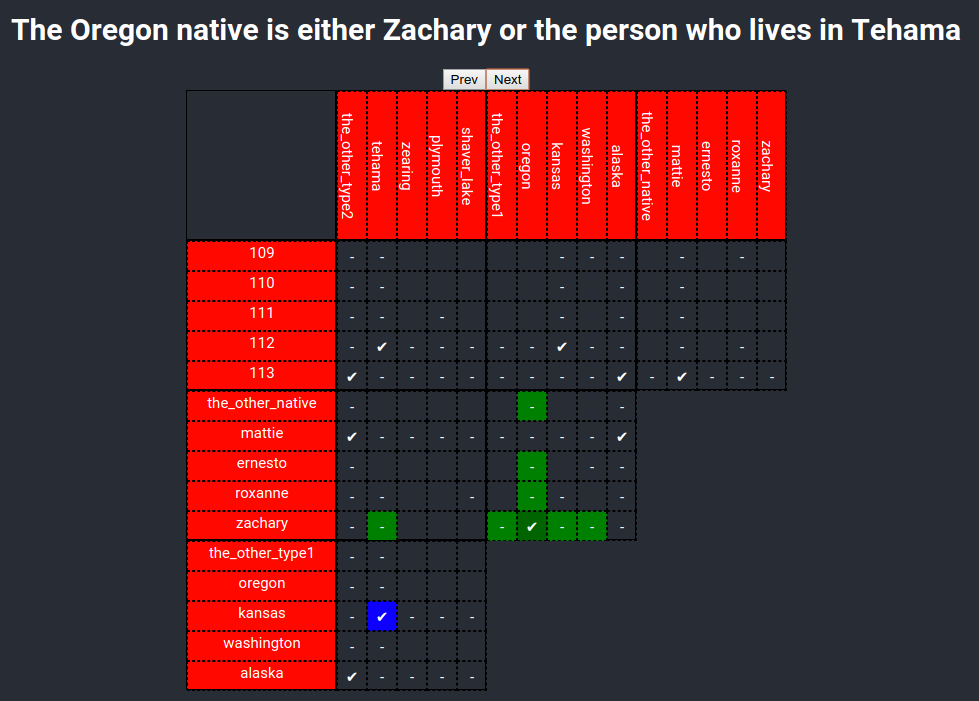
\includegraphics[width=\columnwidth]{fig/screenshot.png}
 \caption{Screenshot of the visualization.}
 \label{fig:screenshot}
\end{figure}






\todo{Something about the visualisation:
Possibilities/Difficulties with NL generation (non-existing verbs for instance)}


\section{Demonstration}\label{sec:demo}
The working of our system is demonstrated on the following website \url{bartbog.github.io/zebra}. This webpage contains for some puzzles: 
\begin{itemize}
 \item All the the clues, and which (minor) modifications to the natural language formulation we implemented. 
 \item The lexicon that is required to parse the puzzles (semi-automatically generated).
 \item The resulting idp theory associated to each of the clues.
 \item Runnable \idp files to either solve the puzzle, or generate the explanations. 
 \item The visualization of the explanation by derivation steps. 
\end{itemize}
The website is still under construction and will be updated with more puzzles in the near future. 


\section{Conclusion}
\todo{Conclude}


\bibliographystyle{aaai}
\bibliography{idp-latex/krrlib,extrarefs}

\end{document}
